\chapter{Проектирование системы дистрибуции программных модулей}
\label{cha:design}

Проектирование системы дистрибуции программных модулей - это сложная задача, ставка при которой делается не только на функциональность, но и на безопасность. 

\section{Выбор архитектуры системы}

Современная разработка ПО основывается на двух основных типах архитектуры: монолитной и микросервисной. Давайте кратко рассмотрим каждый из этих типов. 

Монолитная архитектура представляет собой классическую модель подхода к программному обеспечению, где используется один самостоятельный модуль, функционирующий отдельно от других приложений. Именно поэтому ее и называют "монолитной". Все фрагменты кода и бизнес-функции в такой архитектуре объединены в одной области.

\begin{figure}
  \centering
  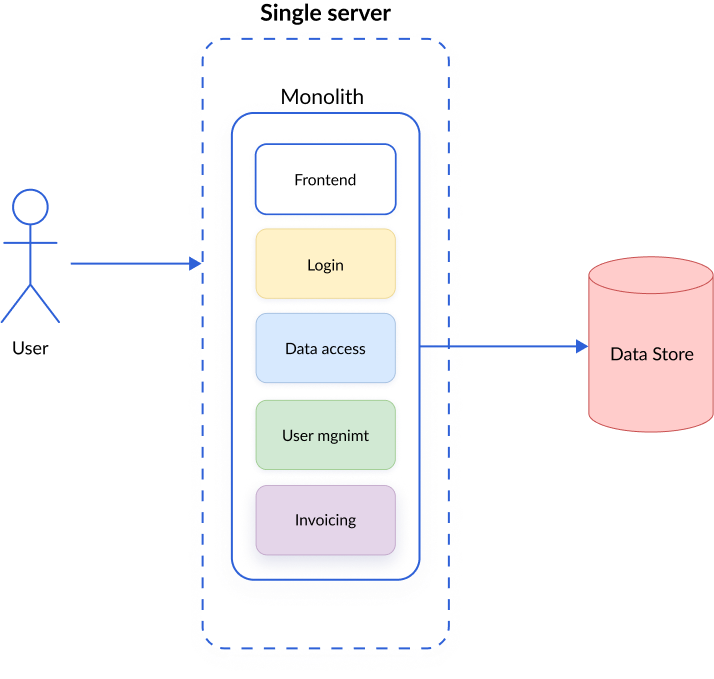
\includegraphics[width=.7\textwidth]{graphics/img/mono.png}
  \caption{Пример монолитной архитектуры}
  \label{fig:mono}
\end{figure}


Микросервисная архитектура - это разделение архитектуры на множество независимо функционирующих служб. Каждая из этих служб имеет свою бизнес-логику и систему управления базами данных (СУБД), служащую определенной цели. Оба эти типа архитектур стоит рассмотреть в контексте сравнения.

\begin{figure}
  \centering
  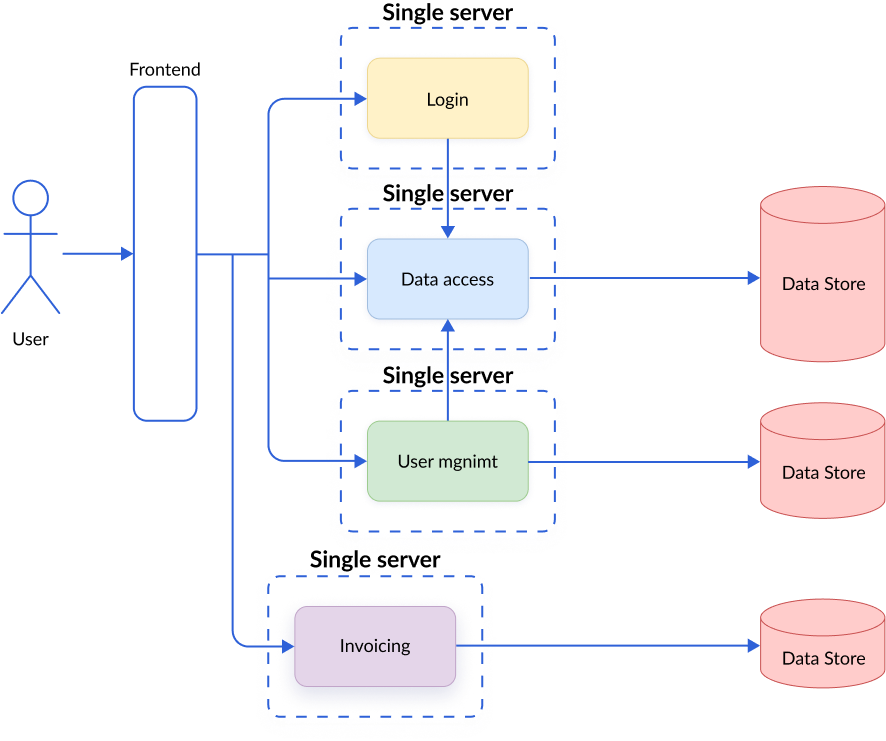
\includegraphics[width=.9\textwidth]{graphics/img/micro.png}
  \caption{Пример микросервисной архитектуры}
  \label{fig:micro}
\end{figure}

Среди недостатков монолитной архитектуры можно выделить плохую масштабируемость, трудность внедрения новых модулей и проблемы при обновлении технологий, так как это может затронуть весь проект, к тому же есть и проблемы с отказоустойчивостью и трудностью в горизонтальной масштабируемости. Однако она проще в развертывании, разработке, тестировании и отладке, чем микросервисная.

Микросервисная архитектура обладает гибкостью: каждая команда может разрабатывать и разворачивать свой сервис независимо, что ускоряет сроки реализации проектов и позволяет выбирать технологии согласно предпочтениям команды. Отказоустойчивость в данном случае - тоже немаловажный плюс, поскольку при сбое одного микросервиса функциональность приложения страдает лишь частично. Недостатками же можно считать большие затраты при разрастании приложения и сложность отладки и координации между разными командами.

Текущий проект работы подразумевает под собой максимальную нагрузку, портируемость и отказоустойчивость. С учетом этого, было решено использовать микросервисную архитектуру, да и существующие системы неспроста являются микросервисными, так как высокие требования делают зависимость от более гибкой системы.

\section{Функциональные возможности системы}

Выробатанными требованиями мы приходим к функциональным возможностям проектируемой системы:

\subsection{Серверная часть системы}

\begin{enumerate}
    \item Загрузка на сервер, отправка пакета (модуля) с сервера.
    \item Управление зависимостями модулей.
    \item Система версий модулей.
    \item Информирование о модулях и их безопасности.
    \item Аутефикация и авторизация на основе JWT.
    \item Реализация открытого API.
    \item Система блокировки и защиты особо критических модулей.
\end{enumerate}

\Abbrev{API}{Application Programming Interface}

\Define{API}{Application Programming Interface ""--- представляет собой набор правил и инструкций, согласно которым различные программы и сервисы могут общаться между собой. Эти правила определяют, как данные и функциональность могут быть переданы от одной программы к другой, как они могут взаимодействовать и обмениваться информацией}

\subsection{Клиентская часть системы}

\begin{enumerate}
    \item Простой и понятный интерфейс через CLI.
    \item Конфигурирование клиентской части.
    \item Управление установленными модулями, включая загрузку, обновление и удаление.
    \item Информирование о модулях и их безопасности.
\end{enumerate}

\section{Микросервис авторизации}

В предложенной работе необходимо разработать микросервис авторизации для системы. Он будет отвечать за следующие функции: 

\begin{enumerate}
    \item регистрацию пользователя.
    \item аутентификацию и авторизацию пользователя.
    \item система сессий через JWT.
    \item система прав у пользователей.
\end{enumerate}

\Abbrev{JWT}{JSON Web Token}
\Define{JWT}{JSON Web Token ""--- руководствующийся открытым стандартом (RFC 7519), представляет собой универсальное средство формирования токенов доступа, рснованный на надежном и широкораспространенном формате JSON, он стал одним из наиболее эффективных и безопасных способов обеспечения эффективной передачи информации между устройствами и серверами в кодированном виде}

\section{API Gateway}
Для полноценного функционирования и получения доступка к микросервисам из любой точки Интернета, необходима единая точка входа, называемая API Gatawey, в качестве которого будет выступать прокси сервер nginx, с модулем поддержки JWT.
\begin{enumerate}
    \item проксирование на необходимые микросервисы;
    \item балансировка нагрузки на запущенные микросервисы;
    \item проверка и прочие действия с JWT;
    \item реализация всех современных стандартов безопасности (CORS и прочие механизмы);
\end{enumerate}

\Define{nginx}{это HTTP-сервер и обратный прокси-сервер, почтовый прокси-сервер, а также TCP/UDP прокси-сервер общего назначения, изначально написанный Игорем Сысоевым}

\Define{CORS-заголовки}{(Cross-Origin Resource Sharing) ""--- это механизм веб-безопасности, который позволяет браузеру загружать данные из стороннего интернет-источника.}

\Define{API Gatawey}{шлюз для API, который упрощает их управление и делает их доступными для клиентов.}

Таким образом, только API Gateway и микросервис авторизации имеют доступ к единому хранилищу, где располагается секретный ключ, используемый для подписи JWT, что повышает безопасность системы в целом. Для предовращения и снижения риска компроментации, ключ рекомендуется менять раз в месяц. 

\section{Микросервис управления пакетами}

\section{CDN}

\Abbrev{CDN}{Content Delivery Network}
\Define{CDN}{Content Delivery Network ""--- это сеть распределенных серверов, которые эффективно передают контент пользователям, основываясь на их географическом положении, источнике контента и сервере с оригинальным содержимым}

В контексте проектирования системы, CDN обеспечивает надежную, высокоскоростную и эффективную доставку модулей от сервера к клиенту. Благодаря CDN, пакеты кода или модулей могут быть быстро и эффективно переданы пользователям независимо от их географического расположения.

Когда разработчик выдает команду для установки определенного модуля, клиент обращается к своему реестру (образу базы данных всех доступных пакетов), который размещен в CDN.

Работая в совокупности с CDN, система дистрибрюции осуществляет следующие функции:

\begin{enumerate}
    \item Обеспечивает надежную и быструю доставку пакетов на компьютеры разработчиков.
    \item Снижает задержку в сети благодаря географическому размещению серверов CDN ближе к пользователям.
    \item Обеспечивает глобальное масштабирование, так как CDN может эффективно обслуживать тысячи запросов по всей России в разных частях и всему миру.
\begin{figure}
  \centering
  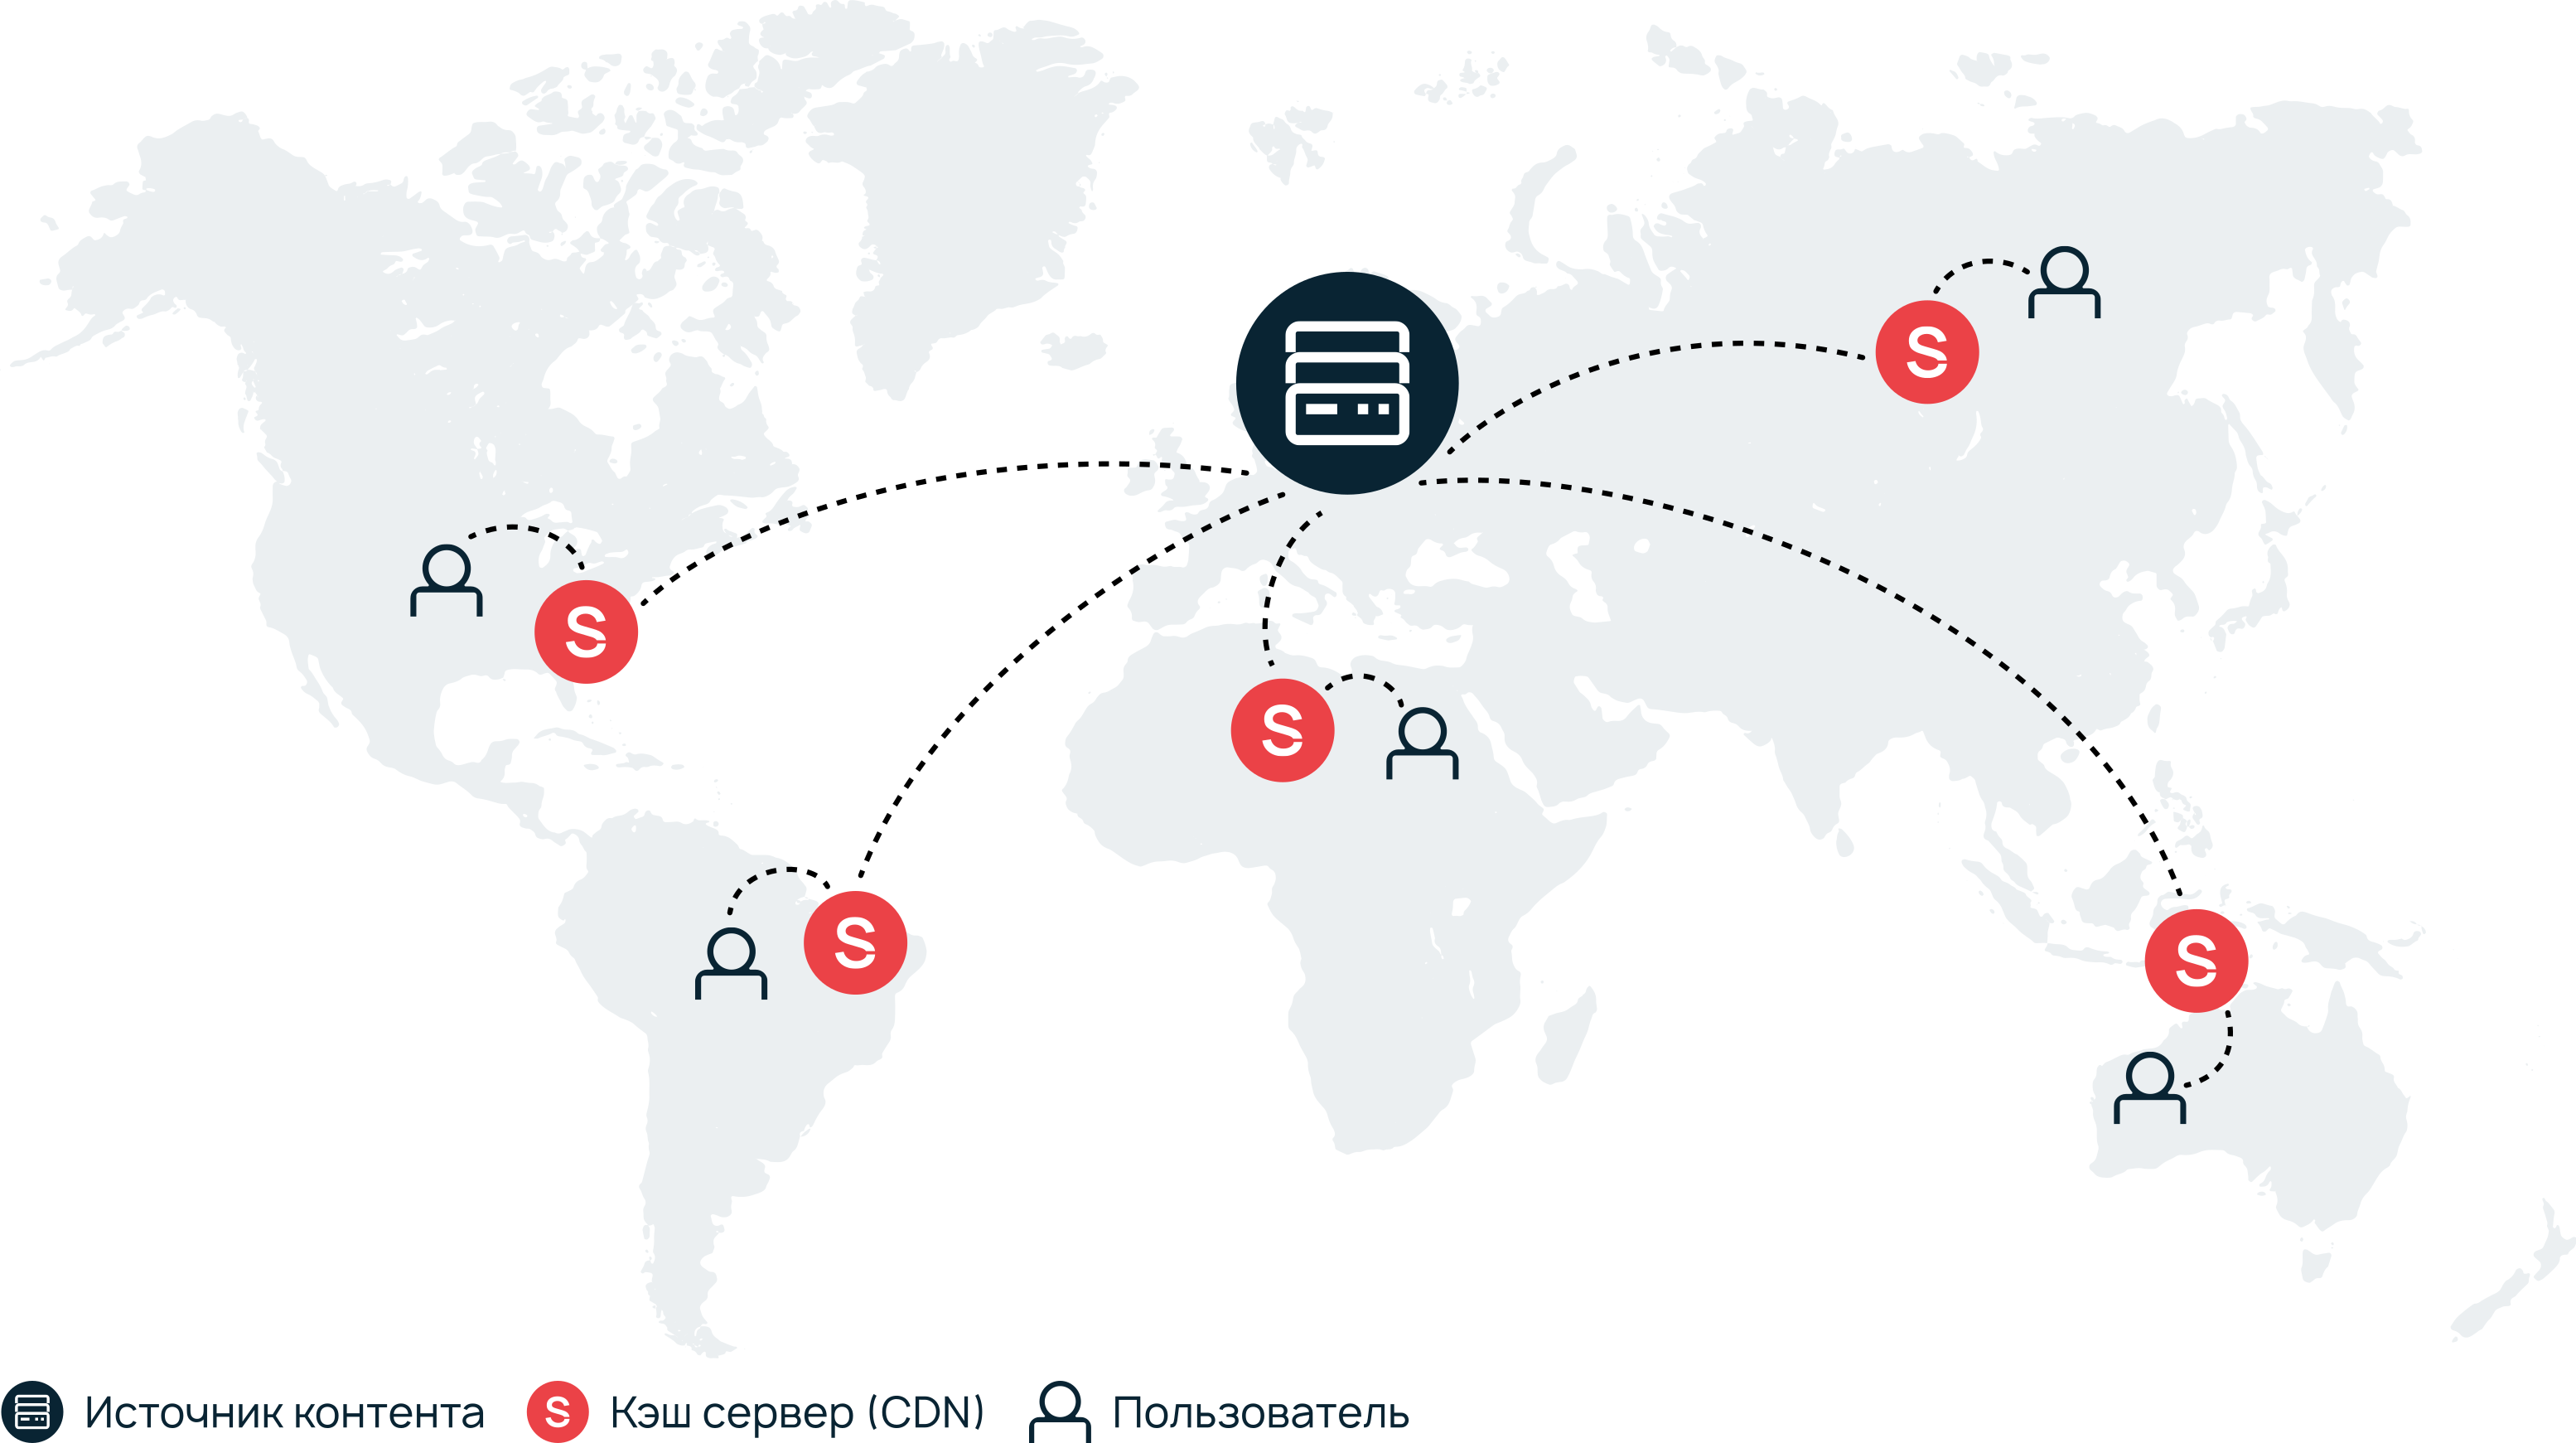
\includegraphics[width=.8\textwidth]{graphics/img/sheme-cdn}
  \caption{Пример визуализации работы CDN}
  \label{fig:mono}
\end{figure}

    \item Увеличивает отказоустойчивость и распределенность системы, поскольку множество точек присутствия CDN могут обслуживать запросы в случае отказа какой-либо из них.
    \item Снижает нагрузку на основные сервисы за счет кеширования.
\end{enumerate}

 При проектировании я решил использовать услуги отечественного провайдера CDN компании Selectel. \cite{cdn:selectel} Выбор данного провайдера был сделан на основе ряда преимуществ, которые он предлагает.

Selectel предоставляет надежные CDN-услуги, что значительно ускоряет загрузку контента, где бы пользователь не находился. Это особенно важно для нашего проекта, так как ориентир на географически распределенную аудиторию и нуждаемся в том, чтобы модули доставлялись быстро и надежно.

\begin{figure}
  \centering
  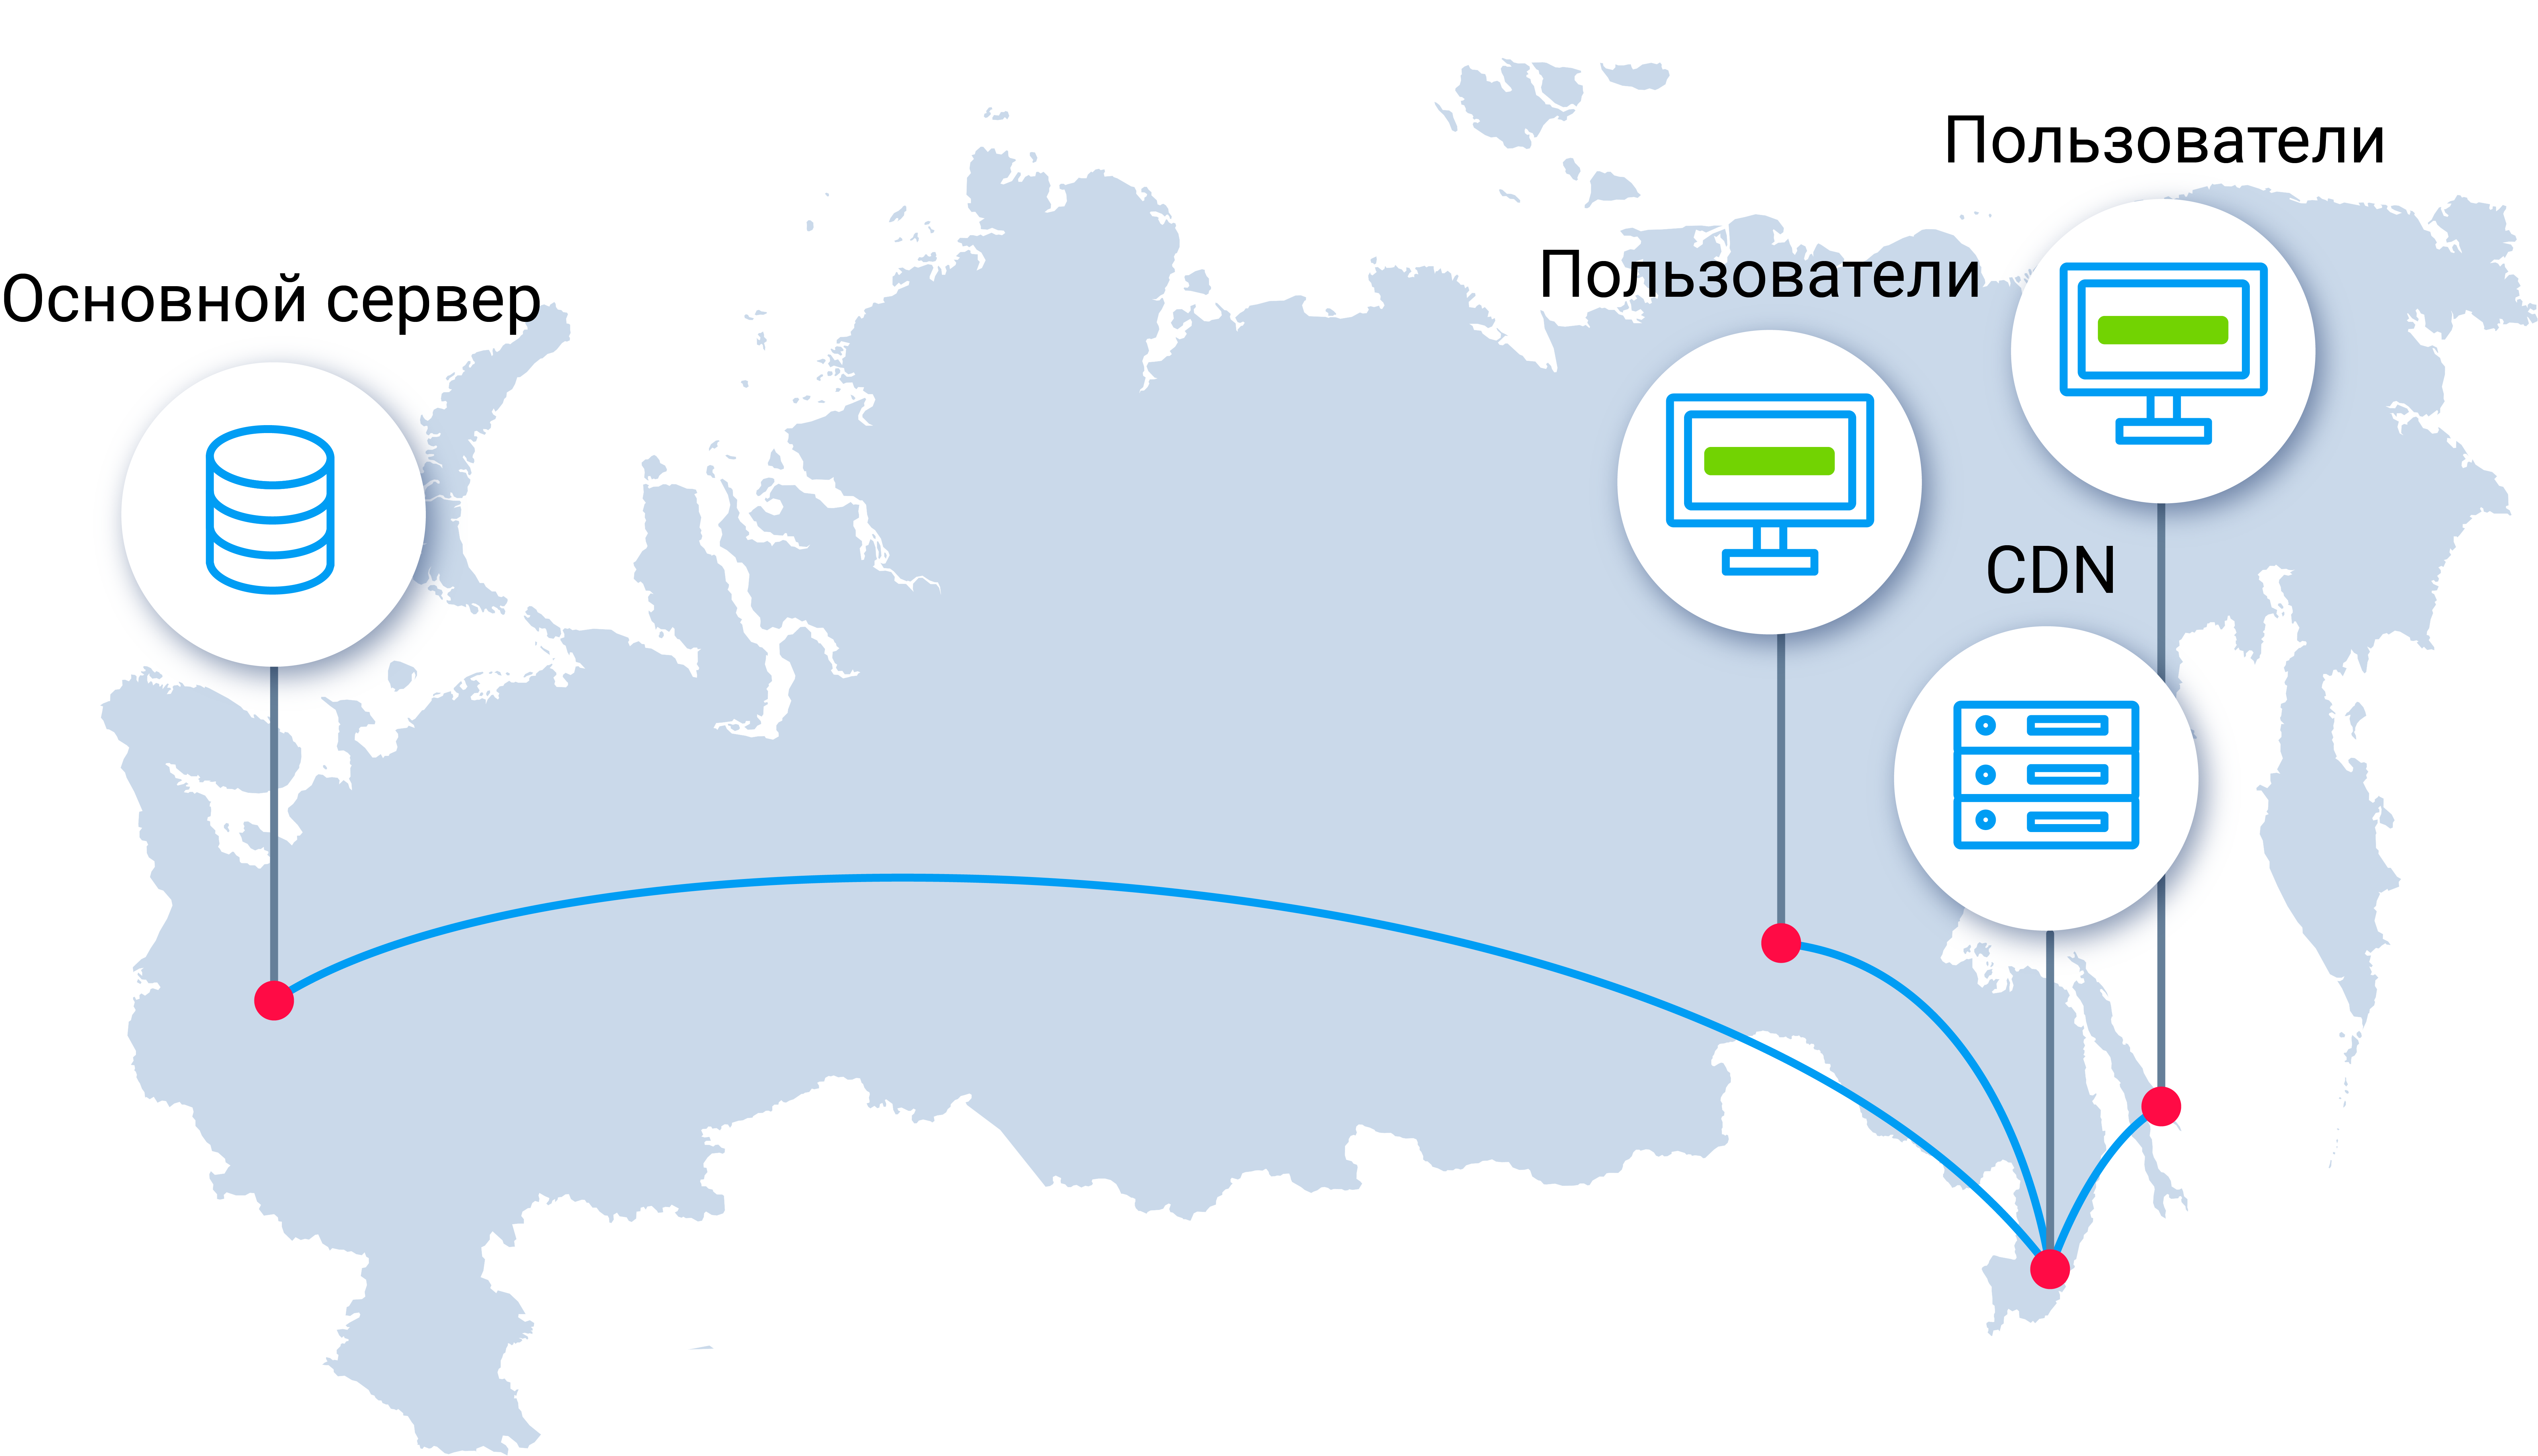
\includegraphics[width=.8\textwidth]{graphics/img/cdn.scheme.5Y4Ydf}
  \caption{Пример визуализации работы CDN в рамках России}
  \label{fig:mono}
\end{figure}

Компания обеспечивает высокую доступность пакетов из-за использования глобальной сети серверов внутри России и по всему миру.

При этом зона собственного покрытия CDN Selectel включает себя такие города \cite{cdn:selectel}, как:
\begin{enumerate}
    \item Россия: Барнаул, Владивосток, Екатеринбург, Иркутск, Казань, Кемерово, Кизляр, Краснодар, Красноярск, Москва, Новосибирск, Орел, Ростов-на-Дону, Санкт-Петербург, Самара, Симферополь, Уфа, Хабаровск, Южно-Сахалинск
    \item Азия: Алматы, Бишкек, Гонконг, Сингапур, Ташкент
    \item Америка: Ашберн, Сан-Паулу
    \item Европа: Амстердам, Минск, Сухум, Франкфурт
\end{enumerate}

Это увеличивает отказоустойчивость проекта и позволяет нам быть уверенными в постоянной доступности модулей для пользователей.

Серверы Selectel обладают высокой пропускной способностью, что среднее время отлика составляет 30 милисекунд \cite{cdn:selectel}, что обеспечивает максимальную скорость передачи данных. Это особенно ценно для системы модульного менеджера, поскольку она имеет дело с большим количеством пакетов, которые должны быть быстро доставлены пользователям.

Кроме того, Selectel уделяет особое внимание вопросам безопасности и защиты данных. Наши пакеты и пользовательские данные хранятся с учетом последних стандартов безопасности, и мы можем быть уверенны в их надежности и защищенности.

При работе с отечественным провайдером у нас также есть возможность получить более оперативную техническую поддержку и консультации по связанным вопросам, что значительно упрощает процесс взаимодействия и решения возникающих вопросов.

В целом, CDN как он встроен в систему, является одним из ключевых факторов обеспечения эффективной и надежной доставки пакетов и модулей, а использование услуг CDN от Selectel, обеспечивает надежность, высокую скорость доставки пакетов, а также высокую степень безопасности данных, что ускоряет время развертывания и обновления проектов, но и снижает время простоя, повышая общую производительность и эффективность процесса разработки ПО.

\section{Оборудование и ОС как часть системы}

Учитывая связанные риски и выроботонные с этим направления, при проектировании учитываем решения на основе русского процессора компании МЦСТ, именованный «Эльбрус-8СВ».

Эльбрус-8СВ - является восьмиядерным промышленным процессором на базе архитектуры Эльбрус (e2k) с использованием длинного командного слова (VLIW), разработанным в России. Он создан для работы в 64-разрядной вычислительной системе и может обрабатывать до 288 гигафлопс двойной точности в одноядерном режиме при частоте 1.5 ГГц, будучи произведенным по техническим нормам в 28 нанометров. Ключевым преимуществом Эльбруса является его отечественное происхождение, что даёт возможность избегать определенных проблем и рисков, связанных с использованием процессоров Intel и AMD. При этом, параметры процессора позволяют полностью закрыть вопрос в потребностях сервисов.

\begin{figure}
  \centering
  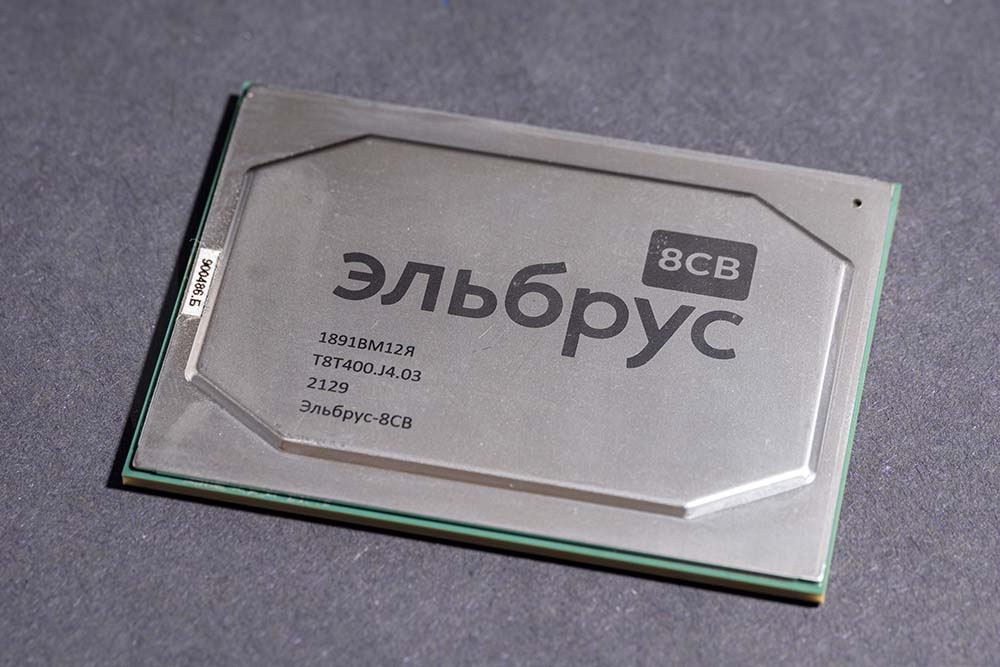
\includegraphics[width=.6\textwidth]{graphics/img/elbrus}
  \caption{Внешний вид процессора компании МЦСТ - Эльбрус-8СВ}
  \label{fig:mono}
\end{figure}

В свете недавних проблем с безопасностью в процессорах Intel и AMD, таких как утечка данных через атаки Spectre и Meltdown, проблемы с микрокодом и другие, использование процессора Эльбрус представляет собой весьма привлекательное решение. Он обладает потенциалом минимизировать тактические и стратегические риски связанные с используемым железом, включая риски иностранных поставок, уязвимости безопасности и ответственность за продукт.

Атаки Spectre и Meltdown стали известны в 2018 году и поставили под угрозу безопасность процессоров Intel, ARM, AMD и некоторых других. Эти атаки используют уязвимости в методах оптимизации работы процессора — так называемой спекулятивной и предсказательной вычислительной системе.

Meltdown и Spectre эксплуатируют «спекулятивное выполнение» \cite{risk:spectual_hack} - функцию, при которой процессор предварительно вырабатывает инструкции, которые могут понадобиться в дальнейшем, чтобы ускорить выполнение кода. Это делает системы уязвимыми, поскольку атакующие могут гипотетически пройти по этим предварительным вычислениями и получить доступ к конфиденциальной информации, которую обычно не должны были бы видеть.

Внедрение исправлений для этих уязвимостей в микрокод процессоров Intel и AMD столкнулось с рядом проблем. Например, первоначальные исправления от Intel вызвали проблемы с перезагрузкой и привели к снижению производительности у некоторых пользователей. Затем Intel выпустил обновленные патчи, чтобы решить эти проблемы. AMD также столкнулась с проблемами, связанными с исправлениями Spectre, но в конечном итоге выпустила серию обновлений микрокода для устранения этих уязвимостей.

\Abbrev{Intel ME}{Intel Management Engine}
При этом, Intel ME, это встроенный модуль микроконтроллера, присутствующий во всех чипсетах Intel с 2006 года, который имеет полный доступ к памяти компьютера, сети и другим частям системы, даже когда компьютер выключен или система спит.

Аналогом Intel Management Engine в мире AMD является AMD Secure Technology, которую ранее называли Secure Processor (или Platform Security Processor, PSP). PSP от AMD также был подвержен уязвимости, схожей у Intel ME \cite{risk:amdpsp}.

Уязвимости Intel ME представляют собой нарушение безопасности из-за незадокументированных возможностей данной части процессора, с возможностью удаленно управлять и исполнять код внутри Intel ME, что и демострируют специалисты компании Positive Technologies \cite{risk:intelme}, показывая возможность выполнения кода даже на выключенном сервере. Эти уязвимости позволяют хакерам возиться с компьютером, обходя встроенные защитные механизмы. По сути, это означает, что злоумышленник может полностью контролировать компьютер с уязвимостью Intel ME, управлять его работой и получать доступ к любым его данным.

Для управления используется AMT, который работает постоянно, жесткий диск — нет, но для изменения кода в  Intel ME жесткого диска не нужен. При этом, обычное ожидание ничем не дает безопасности. При этом у Intel есть технология конфигурации с другого хоста, можно в качестве другого хоста подсунуть взломанный Intel ME, и он заразит соседний сервер в результате, а все сервера «выключены». Аппаратные возможности таких решений настараживают и заставляют отказаться от данных процессоров этих компаний.

Однако российские процессоры Эльбрус не были уязвимы для этих атак. Это объясняется архитектурой и методами оптимизации работы процессора, отличающимися от используемых в Intel и AMD. Конкретно, процессоры «Эльбрус» не используют подобное спекулятивное выполнение и системы управления процессором, а значит, уязвимые атаки не могут быть использованы. \cite{risk:elbrus_no_spectre}

В качестве оптимальной операционной системы, которую можно реализовать на оборудовании Эльбрус с использованием пакетного менеджера, можно рассматривать AstraLinux. Это российский дистрибутив на основе Debian GNU/Linux, который нацелен на создание унифицированной, безопасной и легко управляемой операционной системы, c обеспечением высоким уровенем защиты, что особенно важно при работе с критической инфраструктурой, такие как системы дистрибюции модулей.

Таким образом, сочетание процессора Эльбрус-8СВ и операционной системы AstraLinux действительно представляет собой мощное и экономически эффективное решение для развертывания системы дистрибьюции модулей. Это дает возможность обойти многие потенциальные проблемы, связанные с внешними поставками, уязвимостями и проблемами безопасности.


%%% Local Variables:
%%% mode: latex
%%% TeX-master: "rpz"
%%% End:
